\section{Incidents, problemàtica al desenvolupament i valoració}\label{incidents}

Durant el desenvolupament com es habitual hom es troba amb problemes a resoldre,
alguns d'ells fruit de l'aprenentatge però d'altres deguts a limitacions
de l'entorn ja sigui físic com virtual.

\subsection{Problemàtica física}

El primer problema a afrontar era fer arribar les peces als pas 3 i 4. 
S'entén que aquest fet es intencionat per complicar una mica
més la pràctica. En el nostre cas això ha estat resolt tombant la pinça com ja s'ha exposat en
les seccions anteriors. El fet de tombar la pinça porta una sèrie complicacions 
addicionals. L'una és que el sistema de coordenades de la pinça no està
ubicat perfectament a la zona de contacte on s'agafen les peces, això fa que
s'hagi de fer una petita correcció en \emph{XY} respecte
a la posició quan està perpendicular. Aquesta correcció és veu al codi com una
resta de 17.0 a \emph{Y}, no definit com a \emph{macro} per resignació.

La so\lgem ució no es gaire elegant però si efectiva, tal vegada si el 
treball a realitzar fos més complexe consideraríem intentar moure el sistema
de coordenades al punt correcte, ja sigui amb la funció \texttt{tool}
com fent un càlcul propi a mà i tenint una funció similar a la \texttt{CAM2ROB}
(secció \ref{cam2rob}).

En l'entorn físic també ens hem trobat amb el problema que les peces
tenen restes de cola i vegades s'aferren entre elles movent dues peces a la
vegada, cosa que desbarata totalment l'execució i requereix un reseteig manual
de l'entorn.

S'entén que tots aquests problemes físics són fruit de viure en un món
material amb certes complicacions que, al cap i a la fi, fan la vida un poc més
interessant. Per altra banda si entram en l'apartat de problemes o incidents
en el programari ens trobam amb coses menys justificables.

\subsection{Problemàtica virtual}

El llenguatge de programació del robot es un autèntic desastre, incòmode i
poc pràctic. A classe s'ha comentat que una de les problemàtiques de la robòtica 
industrial és el temps que és té el robot aturat per programar-lo i 
d'aquí que s'inverteixi molt de temps en simuladors, que no poden, entre d'altres, simular
els problemes físics esmentats anteriorment. Així doncs seria molt més
eficaç tenir millors llenguatges que no indueixin a l'error i facilitin
un desenvolupament més ràpid que no pas dedicar-se a simuladors.

Concretament al llenguatge li sobren coses com el numerat de línia,
sobretot que l'entorn no ho faci de manera completament automàtica.
Requerir numerat només fa que s'hagi de pitjar el botó de re-enumeració
cada cop i esperar que es faci el procés, que incomprensiblement tarda
uns 2 o 3 segons.

Al llenguatge també són necessaris més elements, el primordial són
variables locals i crides de funcions amb un fàcil pas de paràmetres,
les variables globals i el \texttt{gosub} indueixen freqüentment a l'error.

Falta de \emph{macros}, en tot programa, i més els que tracten entorns físics,
són necessaris números màgics, aquests poden ser resolts amb una variable
però si són necessaris per la declaració d'un vector tenim un problema,
i més si el llenguatge no permet que aquests siguin dinàmics. És
trist haver de posar números màgics per tot amb un comentari el costat
on aparegui algun identificador per poder-los localitzar al llarg del codi
quan s'ha de realitzar algun canvi.

Tampoc estaria de més el suport de la funció de \texttt{case} amb \texttt{floats} 
o com a mínim l'entorn podria aixecar un advertiment en ser usat, dient que no funciona.

Finalment comentar que el sistema de mostrat d'errors pobre a més de sovint
pràcticament inexistent.

\subsection{Valoració}
Aquests comentaries venen perquè l'algorisme i modelat de la pràctica s'elaboraren
en unes hores. El gruix de temps invertit ha estat ajustant paràmetres del robot i barallant-se
amb el llenguatge i entorn. Així i tot ha estat d'agrair el fet de poder estar amb contact amb un braç
real. Cal dir que tot i així la pràctica ha estat amena i entretinguda, però en aquests
temps convé més ser critic per millorar encara més el que és té, intentant que cada cop la Universitat
sigui un millor lloc per el creixement de l'estudiant.

 \let\thefootnote\relax\footnotetext{
 Aquest document està baix llicència \href{http://creativecommons.org/licenses/by-sa/3.0/}{Creative Commons Atributive Share-Alike 3.0}
 per tant es pot compartir, modificar i distribuir, però citant els autors originals i sense modificar la llicència.
 De la mateixa manera el codi font està baix llicència GNU GPL v3 per part dels dos autors.\bigskip}
\let\thefootnote\relax\footnotetext{El document en versió digital i el codi font el trobareu a \\ \url{https://github.com/bmiro/raiden}\bigskip}
\let\thefootnote\relax\footnotetext{Aquest document i tota la part de la practica que s'ha pogut ha estat desenvolupat emprant programari lliure:}
\let\thefootnote\relax\footnotetext{\href{http://www.tug.org/applications/pdftex/}{\LaTeX} i \href{http://www.tug.org/applications/pdftex/}{Kile} per el text,
\href{http://www.inkscape.org/}{Inkscape} pels diagrames,
\href{http://kate-editor.org/}{Kate} i \href{http://vim.org/}{Vim} per l'edició del codi font.
\href{http://git-scm.com/}{Git} com a sistema de control de versions.
}

\let\thefootnote\relax\footnotetext{
\begin{center}
\begin{tabular}{cc}

\includegraphics[height=35pt,keepaspectratio=true]{diagrames/by-sa.png}
 & 
\includegraphics[height=35pt,keepaspectratio=true]{diagrames/gnu.png}
\end{tabular}
\end{center}
\begin{center}
\begin{tabular}{cccccc}
 
\includegraphics[height=35pt,keepaspectratio=true]{diagrames/latex.png}
 & 
\includegraphics[height=35pt,keepaspectratio=true]{diagrames/kile.png}
 & 
\includegraphics[height=35pt,keepaspectratio=true]{diagrames/inkscape.png}
 & 
\includegraphics[height=35pt,keepaspectratio=true]{diagrames/kde.png}
 & 
\includegraphics[height=35pt,keepaspectratio=true]{diagrames/vim.jpg}
 & 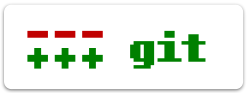
\includegraphics[height=35pt,keepaspectratio=true]{diagrames/git.png}
\end{tabular}
\end{center}
}